%%%%%%%%%%%%%%%%%%%%%%%%%%%%%%%%%%%%%%%%%%%%%%%%%%%%%%%%%%%%%%%%%%%%%%%%%%%%%%%%
%%%%%%%%%%%%%%%%%%%%%%%%%%%%%%%%%%%%%%%%%%%%%%%%%%%%%%%%%%%%%%%%%%%%%%%%%%%%%%%%
%%%%%%%%%%%%%%%%%%%%%%%%%%%%%%%%%%%%%%%%%%%%%%%%%%%%%%%%%%%%%%%%%%%%%%%%%%%%%%%%
\section{Problema \wellposed~ vs. \illposed }

%%%%%%%%%%%%%%%%%%%%%%%%%%%%%%%%%%%%%%%%%%%%%%%%%%%%%%%%%%%%%%%%%%%%%%%%%%%%%%%%
\subsection{Problema \wellposed}
\index{Problema!\Wellposed}
\index{Well-posed}
\begin{definition}[Problema \wellposed:]
\label{def:bem-posto:1}
Conhecido um modelo matemático ou sistema que desejamos manipular para obter uma solução;
indicamos que este é um problema \wellposed~ (do inglês ``well-posed'') 
se cumpre 3 condições\footnote{A definição de um problema \wellposed~ foi realizada pelo matemático J. S. Hadamard, 
para mais detalhes sobre Hadamard ver a Pag. \pageref{elab:Hadamard}.} \cite[pp. 16]{gockenbach2016linear}
\cite[pp. 6]{p2011well}.
\begin{itemize}
\item \textbf{Existência:} Existe uma solução que verifica o sistema.
\item \textbf{Unicidade:} A solução é única.
\item \textbf{Estabilidade:} A solução depende continuamente da saída;
é dizer, pequenas variações na resposta provem de pequenas variações nos dados usados para calcular a resposta.
\end{itemize}
\end{definition}

\begin{example}[Problema \wellposed:]
Conhecido o problema de obter o vetor $\VECTOR{x} \in \mathbb{R}^{N}$,
que cumpre o sistema, $\MATRIX{A}\VECTOR{x}=\VECTOR{y}$,
 tendo como dados o vetor $\VECTOR{y} \in \mathbb{R}^{N}$ e 
a matriz $\MATRIX{A}: \mathbb{R}^{N} \rightarrow \mathbb{R}^{N}$ que carateriza ao sistema.
Falamos que o problema está \wellposed~ se a matriz $\MATRIX{A}$ tem inversa e esta é limitada \cite[pp. 18]{gockenbach2016linear}. 
\end{example}

%%%%%%%%%%%%%%%%%%%%%%%%%%%%%%%%%%%%%%%%%%%%%%%%%%%%%%%%%%%%%%%%%%%%%%%%%%%%%%%%
\subsection{Problema \illposed}
\index{Ill-posed}
\index{Problema!\Illposed}
\begin{definition}[Problema \illposed:]
\label{def:mal-posto:1}
Um problema é chamado \illposed~ (do inglês ``ill-posed'') se não cumpre um o mais das condições que definem a um problema 
\wellposed~ \cite[pp. 18]{gockenbach2016linear}.
Os problemas inversos geralmente são relacionados a um problema \illposed,
pois pelo geral não cumprem uma ou mais das condições para ser catalogados como \wellposed. 
\end{definition}

\begin{example}[Problema \illposed~ sem solução:]
\label{ex:IllPosedNoSolutions}
Conhecido o problema de obter o vetor $\VECTOR{x}\in \mathbb{R}^N$,
que cumpre o sistema,
\begin{equation}
\MATRIX{A}\VECTOR{x}=\VECTOR{y},
\qquad
\MATRIX{A}=
\begin{bmatrix}
1 & 1\\
2 & 1\\
0 & 1
\end{bmatrix}
\qquad
\VECTOR{y}=
\begin{bmatrix}
2\\
3\\
2
\end{bmatrix}.
\end{equation}
Catalogamos este problema como \illposed~ pois não existe um vetor $\VECTOR{x}$
que verifique o sistema $\MATRIX{A}\VECTOR{x}=\VECTOR{y}$.
\end{example}


\begin{example}[Problema \illposed~com múltiplas soluções:]
\label{ex:IllPosedMultiplaSolutions}
Conhecido o problema de obter o vetor $\VECTOR{x}\in \mathbb{R}^N$,
que cumpre o sistema,
\begin{equation}
\MATRIX{A}\VECTOR{x}=\VECTOR{y},
\qquad
\MATRIX{A}=
\begin{bmatrix}
1 & 1\\
1 & 1\\
1 & 1
\end{bmatrix}
\qquad
\VECTOR{y}=
\begin{bmatrix}
2\\
2\\
2
\end{bmatrix}.
\end{equation}
Catalogamos este problema como \illposed~  pois existem múltiplas soluções $\VECTOR{x}$
que cumprem o sistema,
$
\VECTOR{x}=
\begin{bmatrix}
2 & 0
\end{bmatrix}^{\transpose}
+\alpha
\begin{bmatrix}
-1 & 1
\end{bmatrix} ^{\transpose}$,
$ \forall \alpha \in \mathbb{R}$.
\end{example}

\index{Hadamard, Jacques Salomon}
\begin{elaboracion}[title=Jacques Salomon Hadamard (1865-1963), width= 0.99\linewidth]
\label{elab:Hadamard}
\noindent
\begin{minipage}{0.2\linewidth}
\centering
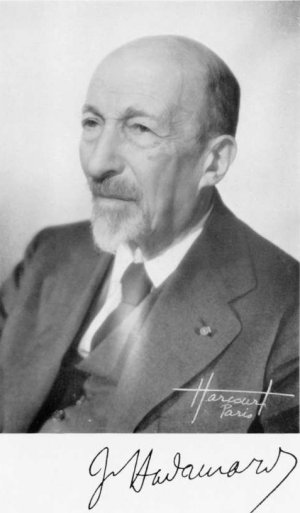
\includegraphics[width=0.98\textwidth]{chapters/notacao/Hadamard2.jpg}
\end{minipage}
\begin{minipage}{0.8\linewidth}
Notável matemático francês  e um membro da Royal Society;
durante seus primeiros anos de vida, 
Jacques se destacou em todas as disciplinas, exceto em matemática;
sua habilidade nesta área melhorou notavelmente após sua admissão no Lycée Louis-le-Grand em 1876;
logo de vários anos, cheios de  grandes realizações acadêmicas, ele completou seu Ph.D. em 1892 
e recebeu o prêmio Grand Prix de Ciências Matemáticas por seu ensaio inovador sobre a função zeta de Riemann
\cite[pp. 326]{agarwal2014creators}.
Entre suas muitas contribuições à matemática está a definição inicial de um problema \wellposed,
e consequentemente a de um problema \illposed~\cite[pp. 9, 132]{p2011well}.
\end{minipage}
\end{elaboracion}

\begin{comment}
\begin{tcbinformation} 
\textbf{Hadamard e os problemas \illposed:} 
O matemático Jacques Salomon Hadamard fez a definição inicial de um problema \wellposed,
e consequentemente a de um problema \illposed; 
ele  indicou como irrelevantes para a física ou para as aplicações do mundo real
a qualquer problema catalogado como \illposed; porém,
quatro décadas após sua declaração esta afirmação ele provou estar errado  \cite[pp. 4]{siddiqi2011mathematics}.
\end{tcbinformation} 
\end{comment}
